\section{Blockchain}
\label{sec:blockchain}

\textit{Blockchain} adalah sekuens dari blok yang menyimpan daftar transaksi lengkap seperti \textit{public ledger} konvensional, dimana setiap \textit{ledger} disimpan pada \textit{node} yang tersebar seperti pada \textit{Distributed Ledger Technology} \parencite{zheng2018blockchain}. Setiap transaksi yang masuk ke dalam sebuah blok akan divalidasi sesuai dengan metrik yang digunakan oleh sistem \textit{blockchain}, dan blok yang memiliki daftar transaksi yang lengkap, ditambah \textit{timestamp} pembuatan blok, nilai \textit{hash} dari blok sebelumnya ("\textit{parent}"), dan sebuah \textit{nonce}, yang adalah sebuah angka acak yang digunakan untuk mekanisme verifikasi \textit{hash}. Konsep ini memastikan integritas dari \textit{blockchain} dimulai dari blok pertama ("\textit{genesis block}") sampai ke blok terakhir, yang terus ditambahkan, karena setiap perubahan data akan membuat nilai \textit{hash} dari sebuah blok berubah, yang harus dipropagasikan ke setiap blok setelahnya. Sebelum ditambahkan ke dalam \textit{blockchain}, setiap blok dan transaksi di dalamnya harus divalidasi oleh mayoritas \textit{node}, menggunakan sebuah mekanisme \textit{consensus} \parencite{nofer2017blockchain}. Mekanisme \textit{consensus} adalah proses dimana mayoritas dari \textit{network validator} menyetujui atau menolak sebuah \textit{state} dari \textit{ledger}. Proses \textit{consensus} mengikuti sebuah kumpulan aturan dan prosedur untuk mempertahankan himpunan fakta yang koheren diantara beberapa \textit{participating nodes}. Terdapat banyak mekanisme \textit{consensus} yang berbeda yang digunakan dalam \textit{blockchain network} yang berbeda. Dalam kasus \textit{Bitcoin}, \textit{ledger} yang dianggap \textit{ledger} yang \textit{valid} adalah \textit{ledger} dengan \textit{chain} terpanjang (\textit{longest chain}) \parencite{swanson2015consensus}.

\begin{figure}[ht]
	\centering
	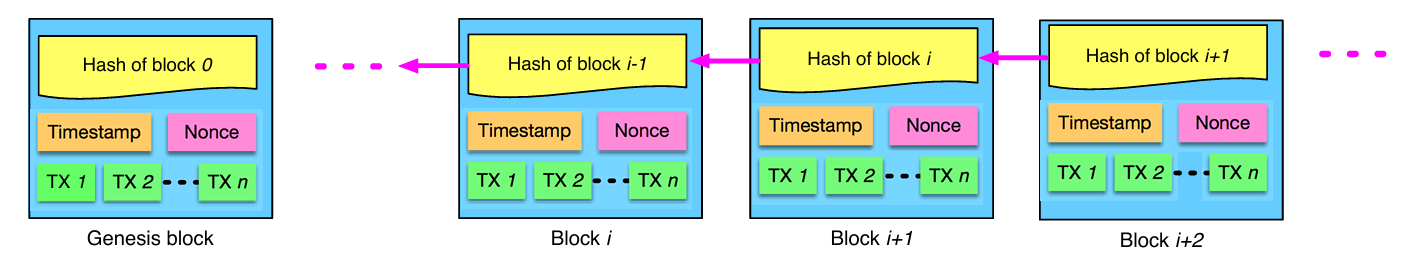
\includegraphics[width=1\textwidth]{resources/chapter-2/struktur-blockchain.png}
	\caption{Struktur blok di dalam \textit{blockchain} \parencite{zheng2018blockchain}}
	\label{image:struktur-blockchain}
\end{figure}

\break

Struktur dari sebuah blok terdiri dari \textit{block header} dan \textit{block body} seperti pada Gambar \ref{image:struktur-blok}. Secara spesifik, \textit{block header} terdiri dari:

\begin{enumerate}
	\item \textit{Block Version}: mengindikasikan set dari aturan validasi yang diikuti.
	\item \textit{Parent Block Hash}: 256-bit \textit{hash} dari blok sebelumnya.
	\item \textit{Merkle Tree Root}: hasil \textit{hash} dari seluruh transaksi pada blok menggunakan mekanisme \textit{Merkle Tree}.
	\item \textit{Timestamp}: \textit{timestamp} saat ini dalam detik sejak 1970-01-01T00:00 UTC.
	\item \textit{nBits}: target \textit{hash} saat ini dalam format \textit{compact}.
	\item \textit{nonce}: \textit{number used only once}, sebuah angka yang digunakan untuk menambahkan tingkat keacakan dari nilai \textit{hash}.
\end{enumerate}

\begin{figure}
	\centering
	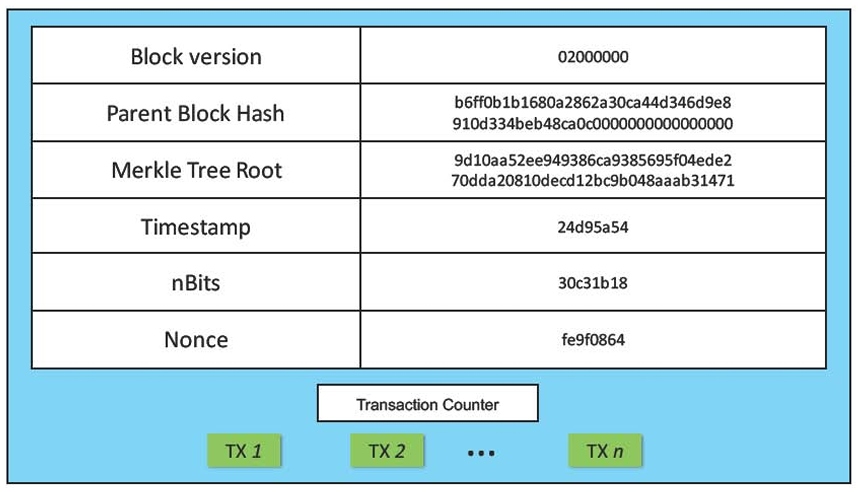
\includegraphics[width=0.7\textwidth]{resources/chapter-2/struktur-block.png}
	\caption{Struktur blok \parencite{zheng2018blockchain}}
	\label{image:struktur-blok}
\end{figure}

\subsection{Blockchain Properties}
\label{subsec:blockchain-properties}

Implementasi dari \textit{blockchain} memunculkan karakteristik dari \textit{blockchain} itu sendiri. Karakteristik ini dapat muncul secara inheren dari sistem dasar dimana \textit{blockchain} di bangun, ataupun muncul karena implementasi spesifik \textit{blockchain}. Beberapa karakteristik penting \textit{blockchain} \parencite{aimar2023extraction}:

\begin{itemize}
	\item \textit{Decentralized}: Tidak ada sebuah entitas terpusat yang mengontrol \textit{network}. Seluruh \textit{participants} mengikuti protokol yang berlaku dan memiliki kontrol yang sama.
	\item \textit{Distributed}: Komputasi dilakukan pada sejumlah \textit{node} atau komputer yang berbeda, yang tersebar dan saling berinteraksi melalui sebuah \textit{p2p network}. Kegagalan sebuah mesin seharusnya tidak mengganggu jalannya protokol.
	\item \textit{Immutable}: Tidak memungkinkan untuk mengubah \textit{history} apapun yang sudah tertulis di dalam \textit{blockchain}. Setelah sebuah blok divalidasi dan dimasukkan ke dalam \textit{blockchain}, tidak dapat dimodifikasi.
	\item \textit{Permissionless}: Semua orang dapat secara aktif berpartisipasi di dalam semua \textit{role} di dalam \textit{network} tanpa perlu meminta \textit{permission}.
	\item \textit{Permissioned}: Mewajibkan seluruh aktor di dalam \textit{network} mendapatkan \textit{authorization} secara eksplisit.
	\item \textit{Transparent}: Semua orang dapat secara independen melihat dan mengunduh data dari \textit{blockchain}.
	\item \textit{Pseudoanonymous}: \textit{Participants} dalam sebuah \textit{blockchain network} tidak perlu membuktikan identitas asli mereka. Seluruh aktivitas di dalam \textit{network} akan disambungkan ke sebuah \textit{address}, bukan identitas asli seseorang.
	\item \textit{Account-based}: \textit{Data} disimpan berdasarkan akun, dan setiap akun memiliki \textit{balance} yang dapat digunakan. Kepemilikan sebuah akun dibuktikan dengan kepemilikan \textit{private key} untuk akun tersebut.
	\item \textit{UTXO-based}: Selain \textit{account-based}, model \textit{UTXO} hanya memiliki konsep dari transaksi. \textit{User} harus membuktikan bahwa mereka memiliki \textit{private key} untuk membuka kunci dari sebuah hasil transaksi untuk menggunakan \textit{balance} yang dimiliki. \textit{Balance} dari seorang \textit{user} adalah penjumlahan seluruh nilai dari hasil transaksi yang dapat dibuka dan digunakan.
\end{itemize}


% \subsection{Contoh Subsubbab}
% \label{subsec:contoh-subsec}



% \subsubsection{Subsubsubbab}
% \blindtext

% \subsubsubsection{sub sub sub sub bab}
% \blindtext

% \begin{table}[h]
% 	\caption{Tabel random}
% 	\vspace{0.25cm}
% 	\begin{center}
% 		\begin{tabular}{|c|c|c|c|}
% 			\hline
% 			Title1 & Title2 & Title3 & Title4  \tabularnewline
% 			\hline
% 			1647   & 1.97   & 0.68   & 1.90 \tabularnewline
% 			2301   & 2.92   & 1.06   & 2.75 \tabularnewline
% 			2969   & 3.23   & 1.16   & 3.78 \tabularnewline
% 			3791   & 4.39   & 1.40   & 4.14 \tabularnewline
% 			4625   & 6.72   & 1.87   & 5.59 \tabularnewline
% 			\hline
% 		\end{tabular}
% 	\end{center}
% \end{table}